\section{Si}
\subsection*{Material ID: mp-cdhjp}
\textbf{Constante Dieléctrica ($\epsilon_{total}$):} 12.13 \\[0.5em]
\begin{table}[h!]
  \centering
  \begin{tabular}{lcc}
    \toprule
    \textbf{Métrica} & \textbf{Lámina (Plate)} & \textbf{Cilindros (Rod)} \\
    \midrule
    Bandgaps ($a/\lambda$) & Ninguno & Ninguno \\
    Resonancias & 36 & 36 \\
    \bottomrule
  \end{tabular}
\end{table}
\begin{figure}[H]
  \centering
  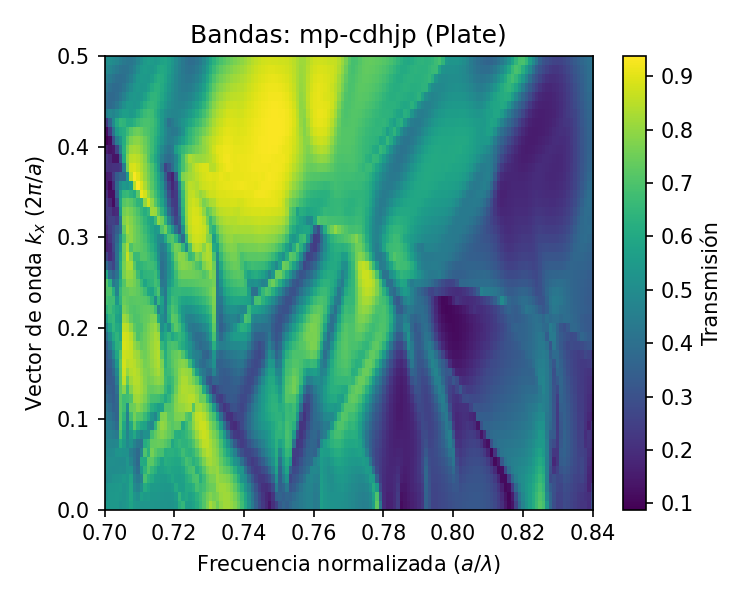
\includegraphics[width=0.48\textwidth]{figures/mp-cdhjp_plate.png}
  \hfill
  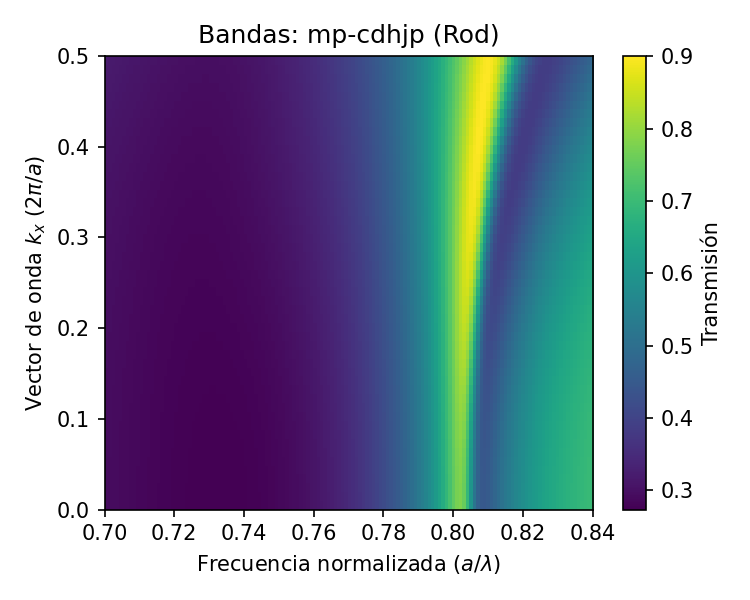
\includegraphics[width=0.48\textwidth]{figures/mp-cdhjp_rod.png}
  \caption{Estructuras de bandas fotónicas para mp-cdhjp. Izquierda: Lámina. Derecha: Cilindros.}
\end{figure}
\vspace{1em}
\hrule
\vspace{1em}
\subsection*{Material ID: mp-ft}
\textbf{Constante Dieléctrica ($\epsilon_{total}$):} 13.00 \\[0.5em]
\begin{table}[h!]
  \centering
  \begin{tabular}{lcc}
    \toprule
    \textbf{Métrica} & \textbf{Lámina (Plate)} & \textbf{Cilindros (Rod)} \\
    \midrule
    Bandgaps ($a/\lambda$) & Ninguno & Ninguno \\
    Resonancias & 36 & 36 \\
    \bottomrule
  \end{tabular}
\end{table}
\begin{figure}[H]
  \centering
  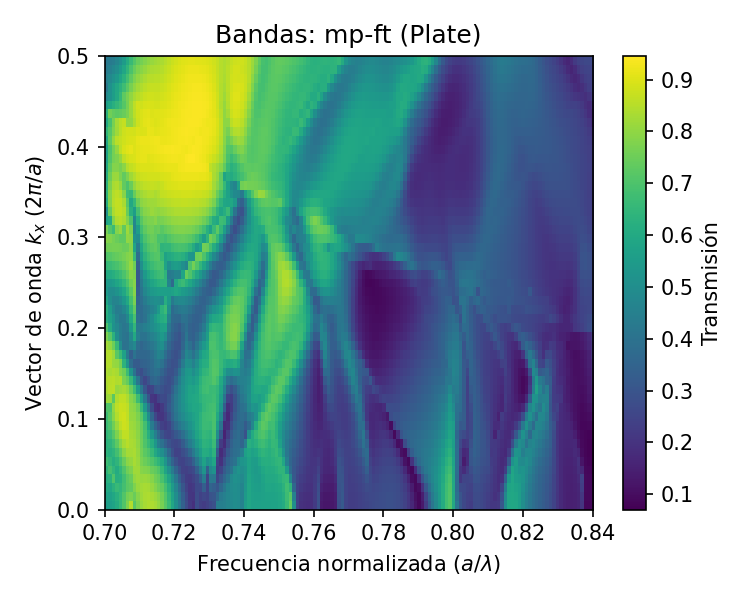
\includegraphics[width=0.48\textwidth]{figures/mp-ft_plate.png}
  \hfill
  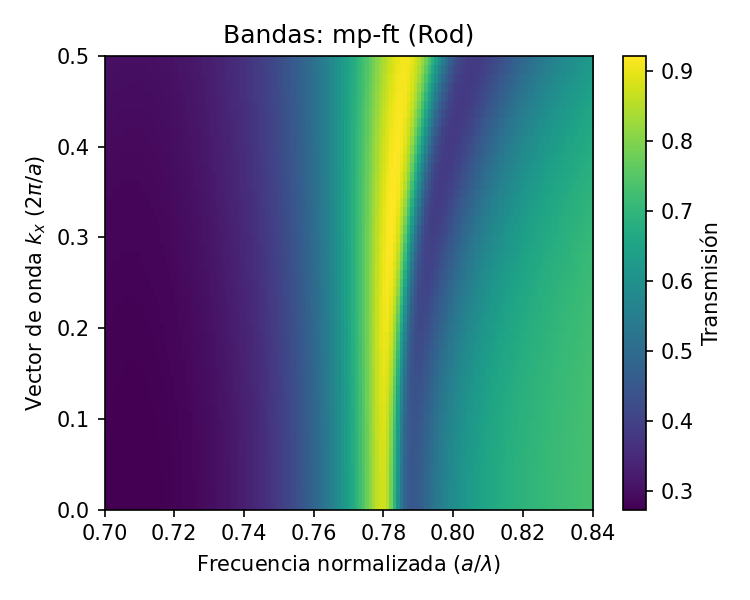
\includegraphics[width=0.48\textwidth]{figures/mp-ft_rod.png}
  \caption{Estructuras de bandas fotónicas para mp-ft. Izquierda: Lámina. Derecha: Cilindros.}
\end{figure}
\vspace{1em}
\hrule
\vspace{1em}
\subsection*{Material ID: mp-gj}
\textbf{Constante Dieléctrica ($\epsilon_{total}$):} 12.75 \\[0.5em]
\begin{table}[h!]
  \centering
  \begin{tabular}{lcc}
    \toprule
    \textbf{Métrica} & \textbf{Lámina (Plate)} & \textbf{Cilindros (Rod)} \\
    \midrule
    Bandgaps ($a/\lambda$) & Ninguno & Ninguno \\
    Resonancias & 36 & 36 \\
    \bottomrule
  \end{tabular}
\end{table}
\begin{figure}[H]
  \centering
  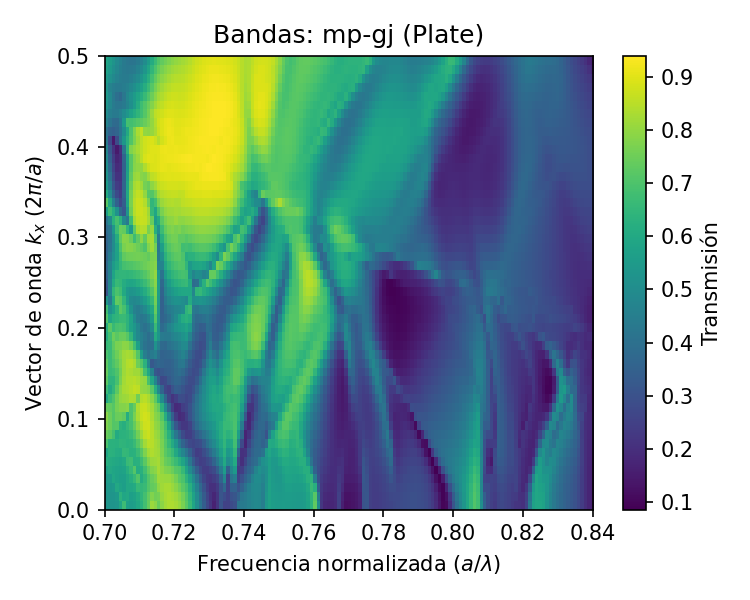
\includegraphics[width=0.48\textwidth]{figures/mp-gj_plate.png}
  \hfill
  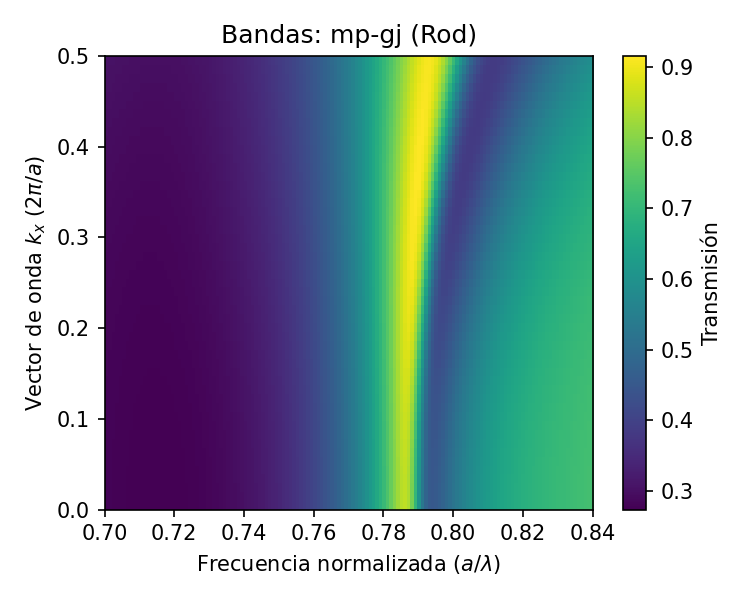
\includegraphics[width=0.48\textwidth]{figures/mp-gj_rod.png}
  \caption{Estructuras de bandas fotónicas para mp-gj. Izquierda: Lámina. Derecha: Cilindros.}
\end{figure}
\vspace{1em}
\hrule
\vspace{1em}

\subsection*{Analisis}

Lo pude encontrar en: \url{https://www.universitywafer.com/silicon-wafer.html} en forma de platina. Lo cual es perfecto pues como pueden ver es la estructura mas interesante. Ademas se puede ver que para los tres tipos de silicio (que se diferencian en el tipo de base en los resultados de The Materials Project) el resultado es practicamente igual en todos los casos. Ahora bien, es supremamente complejo el patron que genera como se puede ver y por tanto distinguir procesos concretos podria resultar muy dificil.


\clearpage
